% !TEX program = xelatex
% 基于 MCP 与 A2A 协议的分布式多智能体协同网络 - 学术海报
\documentclass[25pt, a0paper, portrait]{tikzposter}
\usepackage{xeCJK}
\usepackage{graphicx}
\usepackage{listings}
\usepackage{caption}
\usepackage{subcaption}

% ── 主题 ──
\usetheme{Envelope}
\usecolorstyle{Australia}

\setCJKsansfont{SimHei}
\setCJKmainfont{SimSun}
\setCJKmonofont{SimHei}

% ── 标题区 ──
\title{\parbox{\linewidth}{\centering
    \textbf{\huge 基于 MCP 与 A2A 协议的 \\ 分布式多智能体协同网络}}
}
\author{XXX，XXX，XXX，XXX（团队成员）\texorpdfstring{\\}{}
    指导教师：XXX \texorpdfstring{\\}{}
    北京 XXX 大学 \quad 计算机学院}
\date{}

\begin{document}
\maketitle

\begin{columns}

% ========== 左栏 ==========
\column{0.33}
\block{研究背景与动机}{
    \textbf{问题：} 传统多Agent系统依赖代码级函数调用，Agent间高度耦合，无法体现网络通信的核心思想。

    \textbf{目标：} 构建一个真正\"分布式\"的多智能体旅行规划系统，所有组件通过标准网络协议互联。\\

    \begin{itemize}
        \item \textbf{Agent-to-Agent (A2A)}：Agent间通过TCP/HTTP协议通信
        \item \textbf{Model Context Protocol (MCP)}：Agent与工具服务通过HTTP/JSON-RPC交互
        \item \textbf{服务发现}：注册中心实现动态Agent发现
        \item \textbf{容错设计}：超时、熔断、降级、缓存、重试
    \end{itemize}

    \textbf{应用场景：} 用户输入自然语言旅行需求 $\rightarrow$ 系统自动完成天气查询、景点推荐、酒店预订、交通规划、行李建议。
}

\block{系统架构}{
    \centering
    \begin{tikzfigure}
        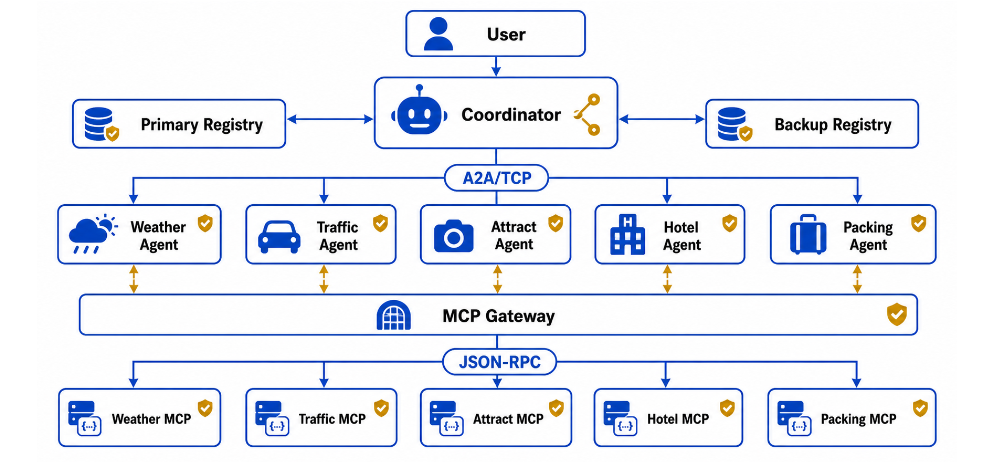
\includegraphics[width=\linewidth]{topology.pdf}
    \end{tikzfigure}
    \vspace{-1em}
    {\small 14个独立进程通过 TCP/HTTP 互联，端口 7000-9060}
}

\block{通信协议栈}{
    \begin{center}
    \begin{tabular}{|c|c|c|}
        \hline
        \textbf{层级} & \textbf{协议} & \textbf{实现} \\
        \hline
        A2A通信 & TCP (4Byte长度前缀 + JSON) & \texttt{common/tcp\_a2a.py} \\
        MCP通信 & HTTP/JSON-RPC 2.0 & \texttt{http.server} \\
        服务发现 & HTTP/REST & Registry \\
        网关层 & JSON-RPC + 缓存/熔断/限流 & \texttt{mcp\_gateway.py} \\
        \hline
    \end{tabular}
    \end{center}
}

% ========== 中栏 ==========
\column{0.34}
\block{核心技术贡献}{
    \textbf{1. 自定义A2A TCP协议} \\
    设计4字节大端长度前缀 + UTF-8 JSON载荷的帧协议，解决TCP粘包问题。

    \textbf{2. 双注册中心高可用} \\
    主备注册中心（7000/7001），Agent同时向两者注册心跳（TTL 6秒），Coordinator自动故障切换。\\

    \textbf{3. MCP Gateway} \\
    \begin{itemize}
        \item TTL缓存（按方法分：天气1天/其他30天）
        \item 每方法并发限流（10并发）
        \item 熔断器（3次失败→熔断10秒→半开探测）
        \item 请求合并（相同并发请求共享上游调用）
    \end{itemize}

    \textbf{4. 实时数据API集成} \\
    高德地图 POI搜索 / 地理编码 / 路线规划 + Open-Meteo 天气预报，Mock数据降级兜底。

    \textbf{5. 智能Agent设计} \\
    \begin{itemize}
        \item \textbf{Coordinator}：LLM动态解析任务→生成DAG→调度Agent
        \item \textbf{酒店Agent}：预算分三档搜索 + 景点坐标重心选址
        \item \textbf{景点Agent}：评分过滤 + 展品识别 + 子景区聚类 + must\_visit模糊匹配
        \item \textbf{交通Agent}：偏好→出行方式自适应 + 实时路线查询
    \end{itemize}
}

\block{DAG工作流引擎}{
    \centering
    \begin{tikzfigure}
        \includegraphics[width=0.9\linewidth]{dag_workflow.pdf}
    \end{tikzfigure}
    \vspace{-1em}
    {\small Coordinator根据Agent依赖关系动态调度：Weather $\rightarrow$ Attraction/Hotel $\rightarrow$ Traffic $\rightarrow$ Packing}
}

% ========== 右栏 ==========
\column{0.33}
\block{实验与验证}{
    \textbf{测试方法：} 20个随机任务并发提交，覆盖不同城市、预算、天数、交通偏好、must\_visit组合。

    \textbf{关键指标：}
    \begin{center}
    \begin{tabular}{|c|c|}
        \hline
        \textbf{指标} & \textbf{结果} \\
        \hline
        任务成功率 & 100\% (20/20) \\
        城市正确率 & 100\% \\
        交通偏好准确 & 100\%（打车/地铁自适应） \\
        并发完成时间 & 216秒（LLM API排队） \\
        MCP实时API成功率 & 95\%+ \\
        must\_visit命中率 & 100\%（含高校/博物馆） \\
        \hline
    \end{tabular}
    \end{center}

    \textbf{典型测试用例：}
    \begin{itemize}
        \item 广州→成都 五星/打车/大熊猫 $\rightarrow$ 全部命中
        \item 杭州→南京 穷游/地铁/中山陵 $\rightarrow$ 全部命中
        \item 厦门 鼓浪屿+厦大 $\rightarrow$ 高校类must\_visit解决
    \end{itemize}
}

\block{网络容错机制}{
    \begin{itemize}
        \item \textbf{超时保护}：MCP 10s / A2A TCP 5s / AMap API 5s
        \item \textbf{降级策略}：API失败后重试3次，全失败→Mock兜底
        \item \textbf{错误隔离}：单Agent失败不影响全局，partial状态返回可用结果
        \item \textbf{注册中心HA}：主节点宕机自动切换备用节点
        \item \textbf{AMap限流保护}：指数退避重试（CUQPS\_EXCEEDED）
    \end{itemize}
}

\block{总结与展望}{
    \textbf{结论：}
    \begin{itemize}
        \item 成功将14个独立进程通过标准网络协议组成完整的分布式多智能体系统
        \item TCP自定义协议、JSON-RPC、注册中心、网关缓存/熔断全链路实现
        \item 20个并发任务100\%成功完成
    \end{itemize}
    \textbf{未来工作：} 跨设备局域网部署、多城市串联路线规划、强化学习优化调度策略。

    \vspace{0.5em}
    {\small \textbf{开源地址：} github.com/fyf-spec/Agent-collaboration-network-on-A2A-MCP}
}

\end{columns}

\end{document}
